\chapter{Una mirada a la evolución humana}\label{ch:g12:human-evolution}

En una capa de ceniza volcánica de tres millones y medio de años, dos
rastros de huellas corren uno junto a otro a lo largo de veintisiete
metros. Los dejaron unas criaturas que caminaban erguidas, apoyando
primero el talón, con el pie arqueado y el dedo gordo alineado con los
demás --- pies como los nuestros --- en una época en la que no existía
ningún cerebro mayor que el de un simio. La marcha erguida llegó
primero, con dos millones de años de ventaja; el cerebro, las
herramientas y el habla vinieron después, y no en línea recta, sino a
lo largo de un matorral de \omterm{def:g10:biodiversity-scales:species}{especies}, casi ninguna de las cuales dejó
descendientes. Este capítulo aplica las herramientas de los dos
capítulos anteriores --- caracteres compartidos, árboles, fechas, \omterm{def:g10:universal-dna:information}{ADN}
--- al linaje que lleva hasta nosotros.

\section{Los humanos entre los primates}

\begin{proposition}[Nuestro lugar en el árbol]\label{prop:g12:human-evolution:place}
Los humanos somos primates: mamíferos con manos prensiles, uñas en
lugar de garras, \omterm{def:g11:the-eye:parts}{ojos} dirigidos hacia delante y un cerebro grande para
su tamaño. Dentro de los primates, los grandes simios --- orangután,
gorila, chimpancé, bonobo, humano --- forman un \omterm{prop:g12:phylogenetic-trees:rules}{clado} y, dentro de él,
el chimpancé y el bonobo son el grupo hermano de los humanos: nuestro
\omterm{def:g10:universal-dna:information}{ADN} se diferencia del suyo en alrededor del 1,2\% de las posiciones, y
el antepasado común de los dos linajes vivió hace unos seis o siete
millones de años, en África. Ese antepasado no era ni un chimpancé ni
un humano; los dos linajes han evolucionado desde entonces.
\end{proposition}
\begin{proof}[Pruebas experimentales]
Las matrices de caracteres y las comparaciones de \omterm{def:g10:universal-dna:information}{ADN} del
\cref{ch:g12:phylogenetic-trees}: todos los \omterm{def:g10:universal-dna:gene}{genes} secuenciados sitúan
al chimpancé más cerca del humano que del gorila, y el \omterm{def:g11:cell-cycle-mitosis:chromosome}{cromosoma} 2
humano es la fusión, extremo con extremo, de dos \omterm{def:g10:universal-dna:information}{cromosomas} que en el
chimpancé siguen separados --- y por eso nosotros tenemos 23 parejas y
ellos 24. El reloj molecular, calibrado con las fechas fósiles de
separaciones más antiguas de primates, data el nodo humano--chimpancé.
\end{proof}

\begin{definition}[El linaje humano]\label{def:g12:human-evolution:lineage}
El \emph{linaje humano}\index{linaje humano} es el \omterm{prop:g12:phylogenetic-trees:rules}{clado} de todas las
\omterm{def:g10:biodiversity-scales:species}{especies} más próximas a los humanos actuales que al chimpancé: todo lo
que desciende del lado humano del nodo de los seis millones de años.
Contiene una \omterm{def:g10:biodiversity-scales:species}{especie} viva, \emph{Homo sapiens}, y una veintena de
\omterm{def:g10:biodiversity-scales:species}{especies} fósiles --- los australopitecos y las varias \omterm{def:g10:biodiversity-scales:species}{especies} del
género \emph{Homo}. Un fósil pertenece a él si muestra caracteres
derivados del linaje: marcha erguida, cara acortada, caninos pequeños
y, más tarde, un cerebro grande y herramientas.
\end{definition}

\section{Los caracteres del linaje}

\begin{proposition}[El bipedismo llegó primero]\label{prop:g12:human-evolution:bipedalism}
El primer carácter derivado del \omterm{def:g12:human-evolution:lineage}{linaje humano} es la marcha habitual
sobre dos piernas. Se ve en el esqueleto: la abertura de la base del
cráneo por la que pasa la médula espinal se sitúa debajo del cráneo y
no detrás, de modo que la cabeza se equilibra sobre una columna
vertical; la columna tiene una doble curva; la pelvis es corta y en
forma de cuenco; los fémures se inclinan hacia dentro hasta la rodilla
y llevan los pies bajo el centro del cuerpo; el pie tiene un arco y el
dedo gordo alineado con los demás, hecho para impulsar y no para
agarrar. Todo eso está presente, con unos pocos rasgos de simio, en
fósiles de cuatro millones de años con cerebros no mayores que el de un
chimpancé.
\end{proposition}
\begin{proof}[Pruebas experimentales]
Los rastros de huellas en la ceniza volcánica, de 3,6 millones de años,
muestran una marcha con zancada, con apoyo del talón y con el pie
arqueado. El esqueleto de una australopiteca de 3,2 millones de años,
completo en un 40\%, tiene una pelvis y una rodilla parecidas a las
humanas y un cerebro de unos \qty{400}{cm^3}. Las bases de cráneo de
esa misma edad tienen la abertura de la médula adelantada, bajo el
cráneo. Los caracteres aparecen en este orden: la marcha y, más de un
millón de años después, el crecimiento del cerebro.
\end{proof}

\begin{omfigure}
\begin{tikzpicture}
  \node[anchor=south west, inner sep=0] (img) at (0,0)
    {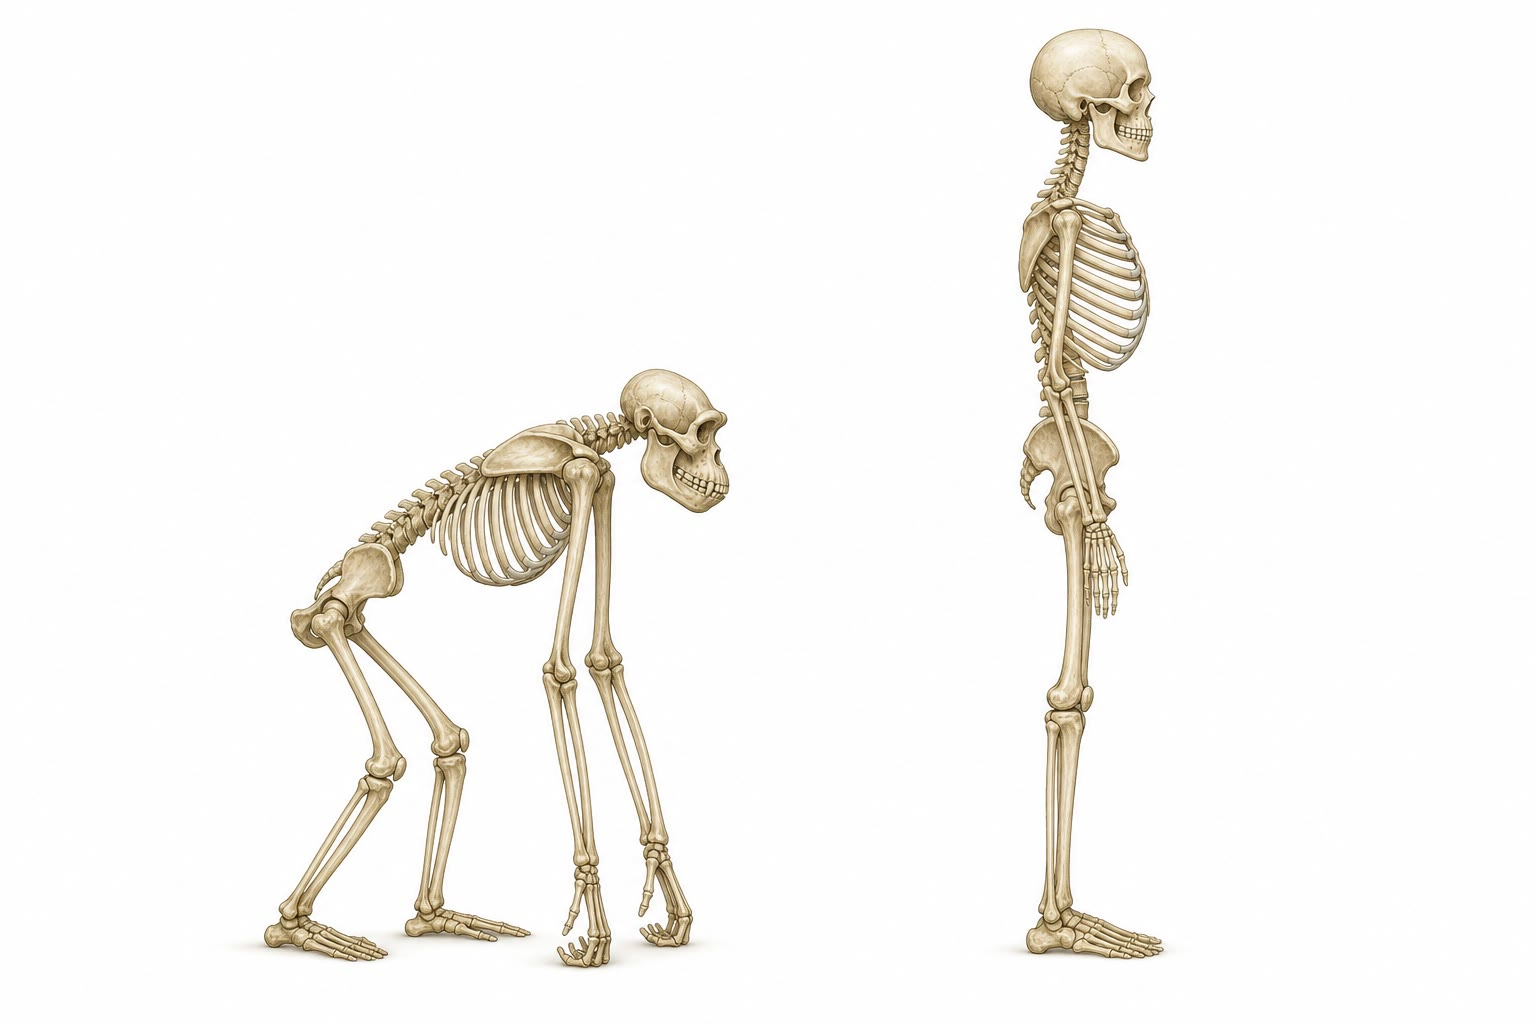
\includegraphics[width=0.56\linewidth]{images/book2/ai/fig-posture-skeletons.jpg}};
  \begin{scope}[x={(img.south east)}, y={(img.north west)},
      every node/.style={font=\scriptsize}]
    \draw[omDef, thick] (0.42,0.585) -- (0.42,0.98) node[above, align=center] {chimpancé: abertura medular\\ en la parte trasera del cráneo};
    \draw[omDef, thick] (0.29,0.50) -- (-0.03,0.62) node[left, align=right] {columna oblicua,\\ cabeza colgada};
    \draw[omDef, thick] (0.23,0.42) -- (-0.03,0.40) node[left, align=right] {pelvis larga\\ y estrecha};
    \draw[omDef, thick] (0.25,0.26) -- (-0.03,0.18) node[left, align=right] {caderas y rodillas\\ dobladas};
    \draw[omDef, thick] (0.70,0.86) -- (1.03,0.90) node[right, align=left] {humano: abertura\\ debajo del cráneo};
    \draw[omDef, thick] (0.68,0.71) -- (1.03,0.68) node[right, align=left] {columna vertical\\ con doble curva};
    \draw[omDef, thick] (0.70,0.54) -- (1.03,0.48) node[right] {pelvis en cuenco};
    \draw[omDef, thick] (0.69,0.32) -- (1.03,0.26) node[right, align=left] {rodillas bajo\\ el tronco};
  \end{scope}
\end{tikzpicture}

{\small Un esqueleto de chimpancé y otro humano de perfil. En el simio,
la médula espinal sale del cráneo por detrás y la cabeza cuelga hacia
delante de una columna oblicua, sobre caderas y rodillas dobladas; en
el bípedo, la abertura está debajo del cráneo, la cabeza se equilibra
sobre una columna vertical de doble curva, la pelvis es corta y en
forma de cuenco y las rodillas quedan bajo el tronco. Una base de
cráneo, una pelvis o una rodilla fósiles pueden leerse para conocer la
marcha.}
\end{omfigure}

\begin{omfigure}
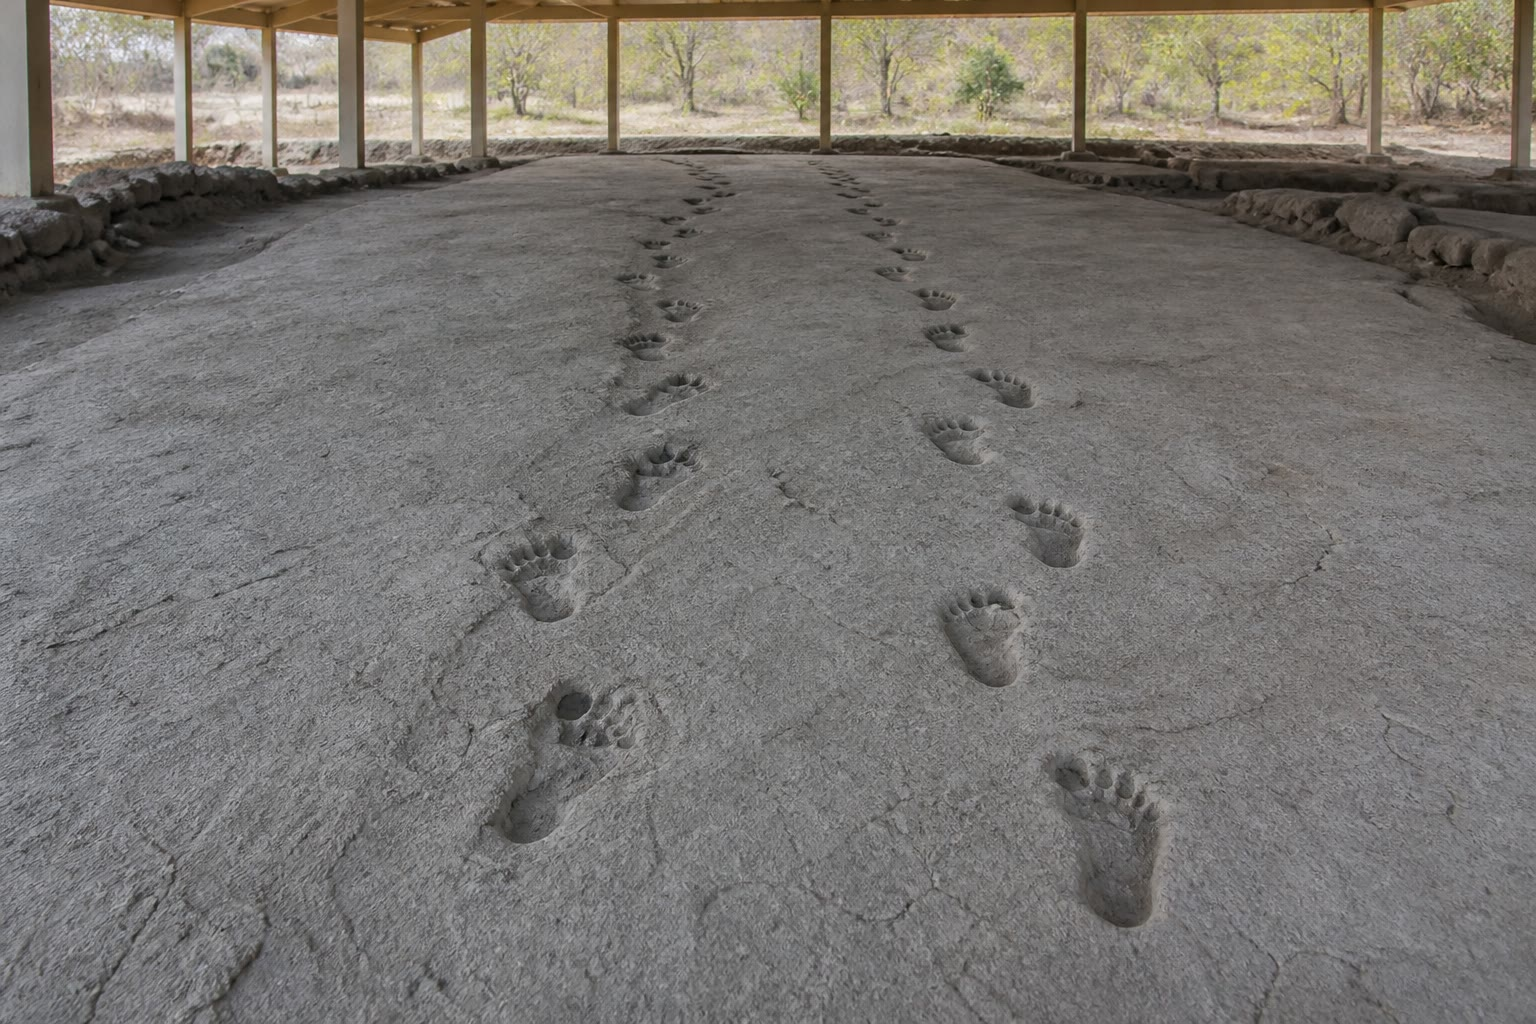
\includegraphics[width=0.6\linewidth]{images/book2/ai/g12-human-footprints.jpg}

{\small Un rastro de huellas conservado en ceniza volcánica endurecida.
Primero el talón, un pie arqueado y el dedo gordo alineado: la huella
de un caminante erguido, dejada millones de años antes de la primera
herramienta de piedra.}
\end{omfigure}

\begin{proposition}[Después el cerebro, las herramientas y la cara]\label{prop:g12:human-evolution:brain}
A partir de hace unos 2,5 millones de años, el linaje muestra un
segundo conjunto de caracteres derivados: un cerebro que crece de
\qty{450}{cm^3} a \qty{1350}{cm^3}, una cara y unas mandíbulas que
menguan bajo él, un mentón y herramientas de piedra --- primero cantos
tallados hasta hacerles un filo, después bifaces trabajados, y después
láminas, puntas y herramientas enmangadas. El fuego está dominado hace
un millón de años, los muertos se entierran hace cien mil y hace
cuarenta mil se pintan imágenes. El cerebro y las herramientas crecen
juntos, y cada uno hace útil al otro, a lo largo de dos millones de
años.
\end{proposition}
\admitted

\begin{omfigure}
\begin{tikzpicture}
\begin{axis}[
  width=0.9\linewidth, height=6cm,
  axis x line=bottom, axis y line=left,
  x dir=reverse, xmin=0, xmax=4.2, ymin=300, ymax=1600,
  xlabel={millones de años atrás}, ylabel={volumen del cerebro ($\mathrm{cm^3}$)},
  xlabel style={font=\small, at={(axis description cs:0.5,-0.12)}, anchor=north},
  ylabel style={font=\small},
  tick label style={font=\small}, xtick={4,3,2,1,0}, ytick={400,800,1200,1600},
  clip=false,
]
\addplot[only marks, mark=*, mark size=2.2pt, omThm] coordinates
  {(3.5,420) (2.5,450) (2.0,600) (1.5,850) (0.8,1000) (0.4,1250) (0.1,1450) (0.05,1350)};
\node[font=\scriptsize, anchor=south] at (axis cs:3.5,450) {australopitecos};
\node[font=\scriptsize, anchor=north] at (axis cs:2.0,570) {\emph{H. habilis}};
\node[font=\scriptsize, anchor=south] at (axis cs:1.5,880) {\emph{H. erectus} temprano};
\node[font=\scriptsize, anchor=north] at (axis cs:0.8,970) {\emph{H. erectus} tardío};
\node[font=\scriptsize, anchor=south] at (axis cs:0.5,1280) {\emph{H. heidelbergensis}};
\node[font=\scriptsize, anchor=east] at (axis cs:0.12,1470) {neandertal};
\node[font=\scriptsize, anchor=north] at (axis cs:0.05,1320) {\emph{H. sapiens}};
\draw[dashed, gray] (axis cs:4.2,400) -- (axis cs:0,400);
\node[font=\scriptsize, gray, anchor=south east] at (axis cs:0.05,405) {chimpancé (hoy)};
\end{axis}
\end{tikzpicture}

{\small Volumen del cerebro de las \omterm{def:g10:biodiversity-scales:species}{especies} del \omterm{def:g12:human-evolution:lineage}{linaje humano} frente a
su antigüedad (medias redondeadas). Plano en los \qty{400}{cm^3} de un
simio durante los dos primeros millones de años de marcha erguida, y
triplicado en los dos siguientes; el cerebro de los neandertales era
algo mayor que el nuestro.}
\end{omfigure}

\begin{omfigure}
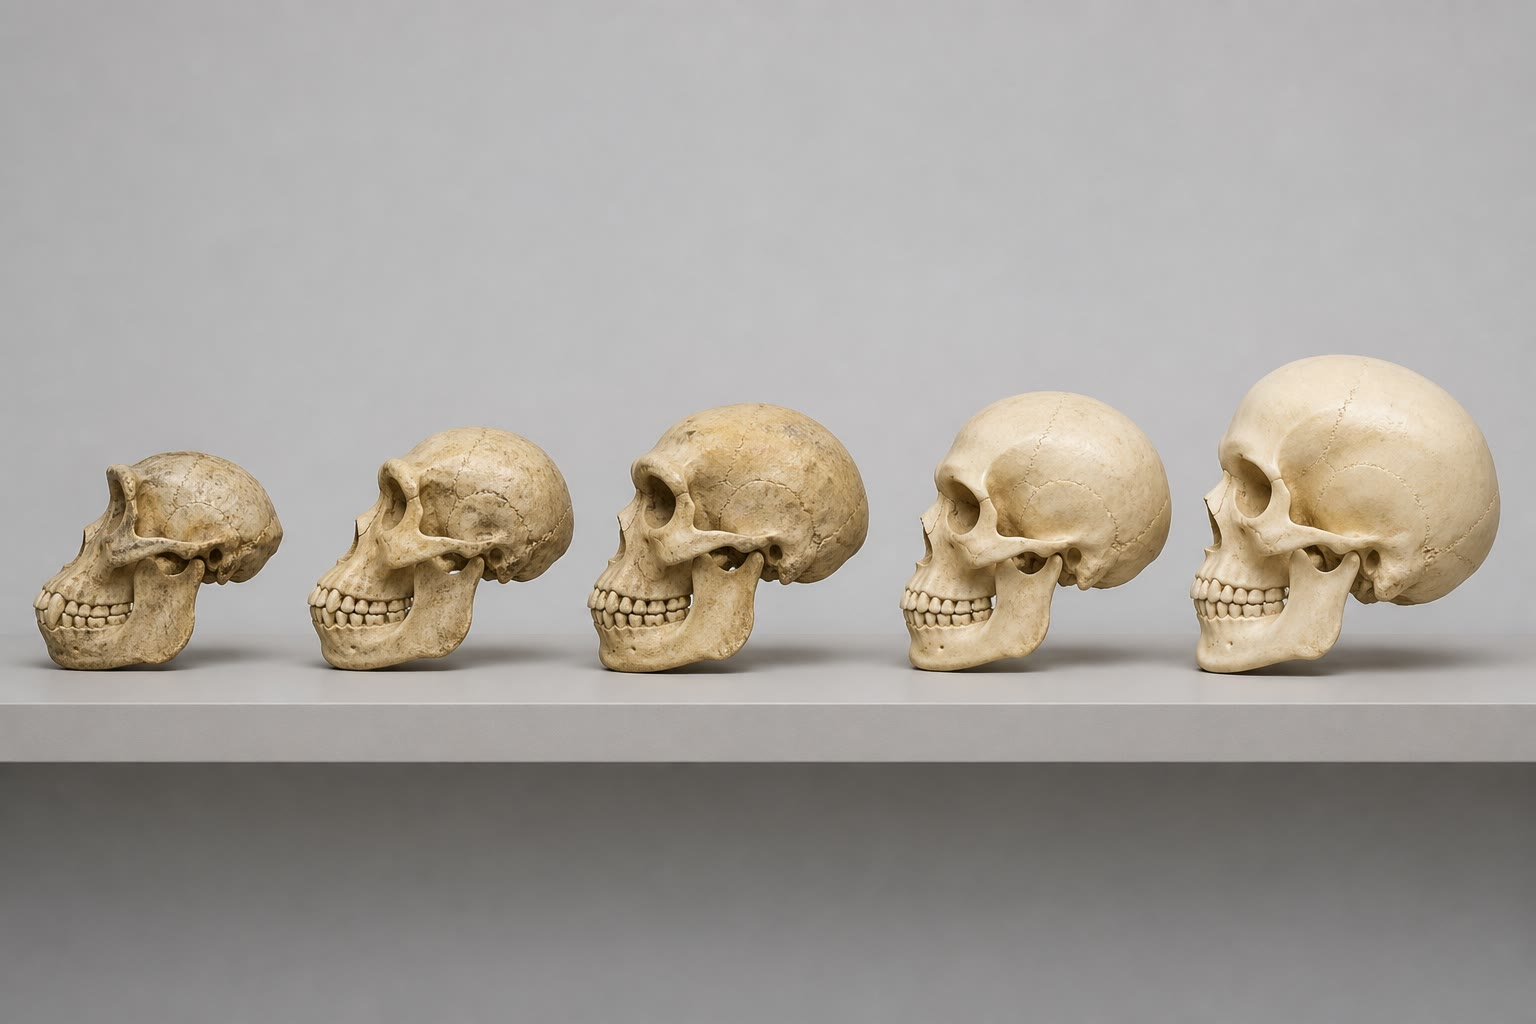
\includegraphics[width=0.66\linewidth]{images/book2/ai/g12-human-skulls.jpg}

{\small Cráneos del linaje de perfil, de un australopiteco a un humano
actual: la caja craneal se hincha, la cara se retira bajo ella, el arco
superciliar se desdibuja y aparece un mentón.}
\end{omfigure}

\begin{example}[Leer un cráneo]\label{ex:g12:human-evolution:skull}
Un cráneo fósil con la abertura medular debajo, una caja craneal de
\qty{450}{cm^3}, mandíbulas grandes y cara saliente es un
australopiteco: erguido y de cerebro pequeño. Uno de \qty{900}{cm^3},
con un arco superciliar potente, la frente huidiza y sin mentón es
\emph{Homo erectus}. Uno de \qty{1400}{cm^3}, con la frente alta, una
cara pequeña metida bajo la caja craneal y mentón es un humano actual.
El orden de esos caracteres en el árbol es el orden en que aparecen en
las rocas.
\end{example}

\section{Un matorral, no una escalera}

\begin{proposition}[Varias especies a la vez]\label{prop:g12:human-evolution:bush}
El \omterm{def:g12:human-evolution:lineage}{linaje humano} no es una sola línea de antepasados y descendientes,
sino un matorral de \omterm{def:g10:biodiversity-scales:species}{especies}, varias de las cuales vivieron a la vez:
dos o tres clases de australopiteco hace dos millones de años junto a
los primeros \emph{Homo}; \emph{Homo erectus} extendido por tres
continentes mientras surgían otras \omterm{def:g10:biodiversity-scales:species}{especies} en África; y hace tan solo
cincuenta mil años, los humanos actuales compartían la Tierra con los
neandertales en Europa, con otra \omterm{def:g12:selection-drift-speciation:population}{población} en Asia y con una \omterm{def:g10:biodiversity-scales:species}{especie} de
cuerpo pequeño en una isla. Casi todas las ramas del matorral acabaron
en extinción; la nuestra es la que queda.
\end{proposition}
\begin{proof}[Pruebas experimentales]
Se encuentran fósiles de \omterm{def:g10:biodiversity-scales:species}{especies} distintas en capas de la misma edad
en los mismos yacimientos. Los restos de neandertales y de humanos
actuales se solapan en Europa durante varios miles de años. El \omterm{def:g10:universal-dna:information}{ADN} de
los neandertales y el de la \omterm{def:g12:selection-drift-speciation:population}{población} asiática, recuperados de sus
huesos, es distinto del nuestro --- y está presente en nosotros: las
personas de fuera de África llevan alrededor de un 2\% de \omterm{def:g10:universal-dna:information}{ADN}
neandertal, y algunas \omterm{def:g12:selection-drift-speciation:population}{poblaciones} del Pacífico un pequeño porcentaje de
la \omterm{def:g12:selection-drift-speciation:population}{población} asiática, la huella de los cruces cuando las \omterm{def:g10:biodiversity-scales:species}{especies} se
encontraron. Las ramas se tocaron antes de terminar.
\end{proof}

\begin{omfigure}
\begin{tikzpicture}[font=\small]
  \tikzset{bar/.style={line width=6pt, line cap=butt}}
  % time axis: 0 at right, 4 Ma at left; 3 cm per Ma
  \draw[->, thick] (0,-0.4) -- (12.6,-0.4);
  \foreach \t/\l in {0/{4}, 3/{3}, 6/{2}, 9/{1}, 12/{0}} { \draw (\t,-0.3) -- (\t,-0.5); \node[anchor=north, font=\scriptsize] at (\t,-0.55) {\l}; }
  \node[anchor=north, font=\scriptsize] at (6.3,-0.95) {millones de años atrás};
  % species bars: (start, end) in Ma -> x = (4 - Ma)*3
  \draw[bar, omDef!60] (0.3,0.4) -- (3.3,0.4); \node[anchor=west, font=\scriptsize] at (3.4,0.4) {\emph{Australopithecus afarensis}};
  \draw[bar, omDef!60] (2.1,1.0) -- (5.7,1.0); \node[anchor=west, font=\scriptsize] at (5.8,1.0) {\emph{A. africanus}};
  \draw[bar, omDef!40] (3.9,1.6) -- (8.4,1.6); \node[anchor=west, font=\scriptsize] at (8.5,1.6) {\emph{Paranthropus}};
  \draw[bar, omProp!60] (4.8,2.2) -- (7.8,2.2); \node[anchor=west, font=\scriptsize] at (7.9,2.2) {\emph{Homo habilis}};
  \draw[bar, omProp!60] (6.3,2.8) -- (11.7,2.8); \node[anchor=west, font=\scriptsize] at (11.8,2.8) {\emph{H. erectus}};
  \draw[bar, omThm!50] (9.9,3.4) -- (11.4,3.4); \node[anchor=east, font=\scriptsize] at (9.8,3.4) {\emph{H. heidelbergensis}};
  \draw[bar, omThm!50] (10.8,4.0) -- (11.88,4.0); \node[anchor=east, font=\scriptsize] at (10.7,4.0) {neandertales};
  \draw[bar, omMeth!70] (11.1,4.6) -- (12.0,4.6); \node[anchor=east, font=\scriptsize] at (11.0,4.6) {\emph{H. sapiens}};
\end{tikzpicture}

{\small Algunas \omterm{def:g10:biodiversity-scales:species}{especies} del \omterm{def:g12:human-evolution:lineage}{linaje humano} y los periodos en los que se
encuentran sus fósiles. En casi todas las fechas coexistieron varias
\omterm{def:g10:biodiversity-scales:species}{especies}; el linaje es un matorral con una sola ramita superviviente.}
\end{omfigure}

\begin{proposition}[Los humanos actuales]\label{prop:g12:human-evolution:sapiens}
\emph{Homo sapiens} apareció en África hace unos 300\,000 años,
reconocible por su cráneo alto y redondeado, su cara pequeña y su
mentón. Unos grupos pequeños salieron de África hace unos 60\,000 años
y, en 50\,000 años, habían llegado a todos los continentes salvo la
Antártida, encontrándose con las \omterm{def:g12:selection-drift-speciation:population}{poblaciones} más antiguas que hallaron
y absorbiéndolas en parte. Todos los humanos vivos descendemos de
aquella \omterm{def:g12:selection-drift-speciation:population}{población} africana: la \omterm{def:g10:biodiversity-scales:biodiversity}{diversidad genética} de toda la \omterm{def:g10:biodiversity-scales:species}{especie} es
menor que la de los chimpancés de una sola región africana, y es máxima
en África y disminuye con la distancia a ella a lo largo de las rutas de
dispersión --- la firma de grupos fundadores sucesivos.
\end{proposition}
\admitted

\begin{omfigure}
\begin{tikzpicture}
\begin{axis}[
  ybar, bar width=14pt,
  width=0.84\linewidth, height=5.2cm,
  axis x line=bottom, axis y line=left,
  ymin=0, ymax=6, ylabel={\% del genoma},
  ylabel style={font=\small},
  symbolic x coords={África subsahariana, Europa, Asia oriental, Melanesia},
  xtick=data, tick label style={font=\small},
  enlarge x limits=0.2, ytick={0,2,4,6},
  legend style={at={(0.03,0.95)}, anchor=north west, font=\small, draw=none},
]
\addplot[fill=omThm!50, draw=omThm] coordinates {(África subsahariana,0.1) (Europa,1.8) (Asia oriental,2.2) (Melanesia,2.0)};
\addplot[fill=omDef!50, draw=omDef] coordinates {(África subsahariana,0) (Europa,0) (Asia oriental,0.2) (Melanesia,3.5)};
\legend{ADN neandertal, ADN de la población asiática}
\end{axis}
\end{tikzpicture}

{\small Porcentaje del genoma heredado de dos \omterm{def:g12:selection-drift-speciation:population}{poblaciones} extinguidas,
por región (redondeado). Las \omterm{def:g12:selection-drift-speciation:population}{poblaciones} que salieron de África se
encontraron con los neandertales y se cruzaron con ellos; las que
llegaron al Pacífico occidental se encontraron además con la \omterm{def:g12:selection-drift-speciation:population}{población}
asiática. Las ramas del matorral intercambiaron \omterm{def:g10:universal-dna:gene}{genes} antes de que
terminaran todas menos una.}
\end{omfigure}

\section{Lo que nos hizo}

\begin{proposition}[Los genes y, después, la cultura]\label{prop:g12:human-evolution:culture}
Los caracteres del linaje surgieron como describen los capítulos
anteriores: \omterm{def:g11:mutations:mutation}{mutaciones}, entre ellas cambios en la regulación de \omterm{prop:g12:diversification-of-life:development}{genes
del desarrollo} (un crecimiento más largo del cerebro, una cara más
corta), clasificadas por la selección en los ambientes de las sabanas
africanas y por la deriva en \omterm{def:g12:selection-drift-speciation:population}{poblaciones} pequeñas. Pero el linaje
añadió un segundo modo de herencia --- el comportamiento transmitido
del \cref{ch:g12:diversification-of-life}, llevado a una escala que
ninguna otra \omterm{def:g10:biodiversity-scales:species}{especie} alcanzó: herramientas, fuego, lenguaje,
cooperación, enseñanza. La cultura se acumula dentro de una vida y pasa
a todos los que la aprenden, y no solo a los descendientes; en los
últimos cien mil años, los cambios que más han importado a los humanos
han sido culturales, y el ambiente en el que la \omterm{def:g10:biodiversity-scales:species}{especie} evoluciona es,
en buena medida, uno que ella misma ha hecho.
\end{proposition}
\admitted

\begin{method}[Situar un fósil]\label{met:g12:human-evolution:placing}
\begin{enumerate}
  \item Data la capa (por la desintegración radiactiva de minerales
        volcánicos o por la edad conocida de los estratos).
  \item Lee la marcha: la posición de la abertura medular, la forma de
        la pelvis y del fémur, el pie.
  \item Mide la caja craneal; fíjate en la cara, en el arco
        superciliar, en el mentón, en los dientes.
  \item Enumera los estados derivados presentes y ausentes y sitúa el
        fósil en el árbol con las reglas del
        \cref{ch:g12:phylogenetic-trees}: como una rama lateral cerca
        del nodo donde encaja su combinación de caracteres, y no como
        ``el antepasado''.
  \item Cuando el hueso se conserva lo bastante bien, lee el \omterm{def:g10:universal-dna:information}{ADN} y
        compáralo con el de las \omterm{def:g12:selection-drift-speciation:population}{poblaciones} vivas.
\end{enumerate}
\end{method}

\begin{remark}[No hay eslabón perdido]\label{rem:g12:human-evolution:link}
La expresión supone una cadena con un hueco; el registro es un matorral
con muchas ramas, casi todas conocidas por unos pocos huesos, y el
``eslabón'' entre nosotros y el chimpancé es un nodo --- una \omterm{def:g12:selection-drift-speciation:population}{población}
extinguida que no era ninguno de los dos --- y no una criatura a medio
camino. Lo que los fósiles sí muestran, en el orden en que las rocas
los conservan, es cada carácter derivado apareciendo a su turno: los
pies, después los cerebros, después las herramientas, después el mentón
--- y en los últimos cincuenta mil años, las obras de una \omterm{def:g10:biodiversity-scales:species}{especie} cuya
evolución es ya, sobre todo, obra suya.
\end{remark}

\section{Ejercicios}

\begin{exercise}[$\star$]\label{exo:g12:human-evolution:1}
¿Qué \omterm{def:g10:biodiversity-scales:species}{especie} viva es el pariente más próximo del humano, y hace cuánto
se separaron los dos linajes?
\end{exercise}

\begin{exercise}[$\star$]\label{exo:g12:human-evolution:2}
Enumera cuatro signos esqueléticos de la marcha erguida.
\end{exercise}

\begin{exercise}[$\star$]\label{exo:g12:human-evolution:3}
En la figura del volumen cerebral, da el volumen de un australopiteco,
del \emph{Homo erectus} temprano y de un humano actual.
\end{exercise}

\begin{exercise}[$\star$]\label{exo:g12:human-evolution:4}
¿Por qué se describe el \omterm{def:g12:human-evolution:lineage}{linaje humano} como un matorral y no como una
escalera?
\end{exercise}

\begin{exercise}[$\star$]\label{exo:g12:human-evolution:5}
¿Dónde y cuándo apareció \emph{Homo sapiens}, y qué muestra el reparto
de la \omterm{def:g10:biodiversity-scales:biodiversity}{diversidad genética} humana?
\end{exercise}

\begin{exercise}[$\star\star$]\label{exo:g12:human-evolution:6}
El \omterm{def:g11:cell-cycle-mitosis:chromosome}{cromosoma} 2 humano corresponde a dos \omterm{def:g10:universal-dna:information}{cromosomas} de chimpancé unidos
extremo con extremo. Explica cómo da cuenta eso de los distintos
números de \omterm{def:g10:universal-dna:information}{cromosomas}, y por qué es una prueba de parentesco y no en
contra.
\end{exercise}

\begin{exercise}[$\star\star$]\label{exo:g12:human-evolution:7}
¿Qué llegó primero en el linaje, la marcha erguida o un cerebro grande?
¿Con cuánta ventaja? Cita las pruebas.
\end{exercise}

\begin{exercise}[$\star\star$]\label{exo:g12:human-evolution:8}
En la figura de la línea de tiempo, ¿qué \omterm{def:g10:biodiversity-scales:species}{especies} coexistían hace dos
millones de años? ¿Y hace 100\,000?
\end{exercise}

\begin{exercise}[$\star\star$]\label{exo:g12:human-evolution:9}
Una persona de ascendencia europea lleva un 2\% de \omterm{def:g10:universal-dna:information}{ADN} neandertal.
Explica qué suceso registra eso y por qué las personas del África
subsahariana no llevan casi nada.
\end{exercise}

\begin{exercise}[$\star\star$]\label{exo:g12:human-evolution:10}
Aplica el \cref{met:g12:human-evolution:placing} a un cráneo con la
abertura medular adelantada, \qty{500}{cm^3} y mandíbulas grandes,
hallado en una capa de 2,8 millones de años.
\end{exercise}

\begin{exercise}[$\star\star$]\label{exo:g12:human-evolution:11}
Explica por qué ``los humanos descienden de los simios'' se enuncia
correctamente como ``los humanos somos simios'', con el vocabulario de
los \omterm{prop:g12:phylogenetic-trees:rules}{clados}.
\end{exercise}

\begin{exercise}[$\star\star\star$]\label{exo:g12:human-evolution:12}
Los neandertales tenían cerebros algo mayores que los nuestros y
fabricaban herramientas complejas y, sin embargo, desaparecieron a los
pocos miles de años de nuestra llegada a Europa. Propón dos hipótesis
compatibles con el capítulo y di qué pruebas las distinguirían.
\end{exercise}

\begin{exercise}[$\star\star\star$]\label{exo:g12:human-evolution:13}
La \omterm{def:g10:biodiversity-scales:biodiversity}{diversidad genética} humana disminuye con la distancia a África a lo
largo de las rutas de dispersión. Explícalo con el efecto fundador del
\cref{ch:g12:selection-drift-speciation} y di qué implica sobre cómo
ocurrió la dispersión.
\end{exercise}

\begin{exercise}[$\star\star\star$]\label{exo:g12:human-evolution:14}
La persistencia de la lactasa, la piel clara en latitudes altas y la
resistencia al paludismo son rasgos humanos que evolucionaron en los
últimos diez mil años. Explica cómo un cambio cultural (la ganadería,
la migración, la agricultura) puede crear la selección que cambia los
\omterm{def:g10:universal-dna:gene}{genes}.
\end{exercise}

\begin{exercise}[$\star\star\star$]\label{exo:g12:human-evolution:15}
``La evolución se ha detenido para los humanos, porque la medicina y la
cultura nos protegen de la selección.'' Discútelo en un párrafo, con la
deriva, los tres rasgos del ejercicio anterior y el significado de la
selección.
\end{exercise}

\section{Problema: Los caminantes de la ceniza}

\begin{problem}[{Problema de fin de semana --- dos rastros de huellas
leídos para deducir la marcha, la estatura y la velocidad; una fila de
cráneos medidos; y el ADN de una estudiante viva rastreado hasta tres
poblaciones}]
\label{pb:g12:human-evolution:1}
Dos rastros de huellas, de 3,6 millones de años, corren paralelos a lo
largo de \qty{27}{m}. Rastro A: huella de \qty{21.5}{cm} de largo,
zancada (de una huella a la siguiente del mismo pie) de \qty{0.95}{m}.
Rastro B: largo \qty{18.5}{cm}, zancada \qty{0.80}{m}. En los humanos
actuales, el pie mide alrededor del 15\% de la estatura de pie, y una
zancada de andar de unas 0,8 veces la estatura corresponde a un paso
lento.

\medskip
\noindent\textbf{Parte I --- Las huellas.}
\begin{enumerate}
  \item Estima la estatura del caminante A y la del caminante B.
  \item Compara cada zancada con 0,8 veces la estatura. ¿Andaban o
        corrían?
  \item Las huellas muestran un talón profundo, un arco y un dedo gordo
        paralelo a los demás. ¿Qué muestra cada rasgo sobre el pie y
        sobre la marcha?
  \item Un chimpancé que camina erguido deja huellas de planta plana y
        dedo gordo divergente, y no puede mantenerlo mucho rato. ¿Qué
        caracteres de la
        \cref{prop:g12:human-evolution:bipedalism} establecen los
        rastros para quienes los dejaron, y cuáles quedan sin conocer?
  \item Los fósiles más cercanos de esa misma edad tienen cerebros de
        \qty{400}{cm^3}. ¿Qué zanja la combinación --- estos pies, ese
        cerebro --- sobre el orden de los caracteres del linaje?
\end{enumerate}

\medskip
\noindent\textbf{Parte II --- Los cráneos.}
Cinco cráneos, con el volumen de la caja craneal, la edad y sus
rasgos: 1: \qty{450}{cm^3}, 3,0 millones de años, cara saliente, sin
mentón. 2: \qty{650}{cm^3}, 1,9 millones de años, cara más pequeña.
3: \qty{950}{cm^3}, 1,0 millones de años, arco superciliar potente, sin
mentón. 4: \qty{1450}{cm^3}, 60\,000 años, arco superciliar potente,
sin mentón, cráneo largo y bajo. 5: \qty{1350}{cm^3}, 30\,000 años,
frente alta, mentón.
\begin{enumerate}[resume]
  \item Asigna cada cráneo a un grupo de la figura de la línea de
        tiempo.
  \item Representa, o describe, el volumen cerebral frente a la edad de
        los cinco. ¿En qué intervalo crece más deprisa el volumen?
  \item El cráneo 4 es mayor que el 5. ¿Identifica el volumen cerebral
        por sí solo a un humano actual? ¿Qué caracteres sí lo hacen?
  \item Los cráneos 4 y 5 se solapan en el tiempo. ¿Qué dice el
        capítulo sobre la relación entre sus dos \omterm{def:g12:selection-drift-speciation:population}{poblaciones}, y qué
        pruebas la apoyan?
  \item El cráneo 1 y las huellas de la Parte I podrían pertenecer a la
        misma \omterm{def:g10:biodiversity-scales:species}{especie}. Explica por qué esa \omterm{def:g10:biodiversity-scales:species}{especie} es un
        \emph{pariente} parecido a un antepasado y no un antepasado
        demostrado, en el lenguaje del \cref{ch:g12:phylogenetic-trees}.
\end{enumerate}

\medskip
\noindent\textbf{Parte III --- El genoma de la estudiante.}
Se compara el genoma de una estudiante de ascendencia europea y
melanesia con los de los neandertales y los de la \omterm{def:g12:selection-drift-speciation:population}{población} asiática
extinguida: el 1,6\% coincide con el genoma neandertal y el 1,8\% con
el asiático.
\begin{enumerate}[resume]
  \item Explica qué significa una coincidencia del 1,6\% y qué suceso
        registra.
  \item Compara sus cifras con el diagrama. ¿Cuál de sus \omterm{def:g12:selection-drift-speciation:population}{poblaciones}
        ancestrales aportó cada parte?
  \item Si los cruces ocurrieron hace 50\,000 años y una generación son
        25 años, ¿cuántas generaciones la separan del suceso? ¿Por qué
        no se ha diluido la parte hasta desaparecer?
  \item Dos linajes aportaron \omterm{def:g10:universal-dna:gene}{genes} al suyo aunque se los llame
        \omterm{def:g10:biodiversity-scales:species}{especies}. ¿Qué dice eso sobre el límite de \omterm{def:g10:biodiversity-scales:species}{especie} del
        \cref{ch:g12:selection-drift-speciation} en aquel momento?
  \item Su \omterm{def:g10:universal-dna:information}{ADN} mitocondrial es del tipo humano actual, como el de todas
        las personas vivas. ¿Qué muestra eso sobre la dirección o sobre
        la suerte de los cruces?
\end{enumerate}

\medskip
\noindent\textbf{Parte IV --- El reloj y el matorral.}
\begin{enumerate}[resume]
  \item El \omterm{def:g10:universal-dna:information}{ADN} humano y el del chimpancé se diferencian en un 1,2\%; el
        reloj de los primates del \cref{ch:g12:phylogenetic-trees} corre
        a un 0,27\% por millón de años. Data el antepasado común.
  \item Los fósiles más antiguos conocidos del \omterm{def:g12:human-evolution:lineage}{linaje humano} tienen de
        6 a 7 millones de años. ¿Es eso coherente con tu fecha?
  \item Enumera las \omterm{def:g10:biodiversity-scales:species}{especies} de la línea de tiempo que estaban vivas
        hace un millón de años y di cuántas de ellas tienen
        descendientes vivos.
  \item Explica por qué los últimos cien mil años del linaje se
        describen mejor con el cambio cultural que con los caracteres
        de este capítulo.
  \item Enuncia el resultado: la estatura y la marcha del caminante A,
        el orden en que aparecieron los pies, el cerebro y el mentón, y
        el número de \omterm{def:g12:selection-drift-speciation:population}{poblaciones} extinguidas cuyos \omterm{def:g10:universal-dna:gene}{genes} lleva la
        estudiante.
\end{enumerate}
\end{problem}
